\documentclass[10pt,twocolumn]{article}

% use the oxycomps style file
\usepackage{oxycomps}

% usage: \fixme[comments describing issue]{text to be fixed}
% define \fixme as not doing anything special
\newcommand{\fixme}[2][]{#2}
% overwrite it so it shows up as red
\renewcommand{\fixme}[2][]{\textcolor{red}{#2}}
% overwrite it again so related text shows as footnotes
%\renewcommand{\fixme}[2][]{\textcolor{red}{#2\footnote{#1}}}

% read references.bib for the bibtex data
\bibliography{references}

% include metadata in the generated pdf file
\pdfinfo{
    /Title (Tutorial on Unity movement)
    /Author (Nico Cantrell)
}

% set the title and author information
\title{Tutorial on Unity movement}
\author{Nico Cantrell}
\affiliation{Occidental College}
\email{ncantrell@oxy.edu}

\begin{document}

\maketitle
\section{Introduction}

For my comps project, I am creating a tool that allows users to learn advanced movement techniques
in certain games, specifically bunny hopping. Bunny hopping is a unique mechanic first found in the source engine, the game engine used for Counter-Strike. It involves the user initiating a jump as
soon as their character touches the ground to minimize the effect that drag has on their character and conserve their momentum. Bunny hopping is present in many games, however it is especially effective in counter-strike as the strafe speed, the speed at which a character moves left and right, is faster in the air than moving forward. As such, the fastest way to move forward in this game is to alternate moving left in the air and moving right in the air with bunny hops in between. This process is complicated to learn, especially for those who have not been in the gaming space for a significant amount of time, and can be a barrier to entry for certain users.

In order to create a tool that can guide users through the process of learning how to bunny hop, I need to understand exactly how the source engine movement works and must be able to design a movement system that closely resembles it for the trainer to be useful. As such, I am following a tutorial that teaches you to implement a basic first-person controller into Unity. I am supplementing that tutorial with several pieces of documentation about the source engine movement to refine this basic movement. The goal of the tutorial is not just to implement a first-person controller but understand what each component does and how each component can be manipulated to enhance your vision for a videogame.

\section{Methods}


The tutorial I followed\cite{UnityTutorial} used Unity as its engine, so I started by downloading and installing Unity. I created a new blank project and created a capsule object for the player and scaled a cube to serve as the floor, shown in figure 1. The first part of the tutorial focuses on implementing first-person camera control. This is done by processing the X and Y input of the mouse and then mapping that both to the camera movement and the player object's orientation changing. In Unity, objects and their basic properties are controlled in the Unity editor shown in figure 2 while more complex functionality is created using C\text{\#} scripts. In order to implement this camera control feature I wrote a script called PlayerCam.cs that takes the x and y Sensitivity, a Transform object and the current x and y rotation of the object. In unity, Transforms are child objects of 3d objects that store that parent object's position, scale and rotation. Storing this information in a child object allows other scripts and objects to alter or mimic changes in position or rotation with the original object. For the PlayerCam script, this means that the camera object can exactly copy the position and rotation of the player despite being a different object. The PlayerCam script locks the cursor to the middle of the screen, makes it invisible and copies the rotation of the camera to the player.

Next, the tutorial covers the setup for the player character in the Unity environment. First there are two parent objects called CameraHolder and Player. CameraHolder has a child camera object PlayerCam that we add our PlayerCam.cs script to. Player has a PlayerObj child which is the capsule object that represents the player in space, the orientation Transform object that keeps track of the player and the CameraPos object that keeps track of the position of the camera as it is slightly higher than the center positon of the actual player.
\begin{figure}
    \centering
    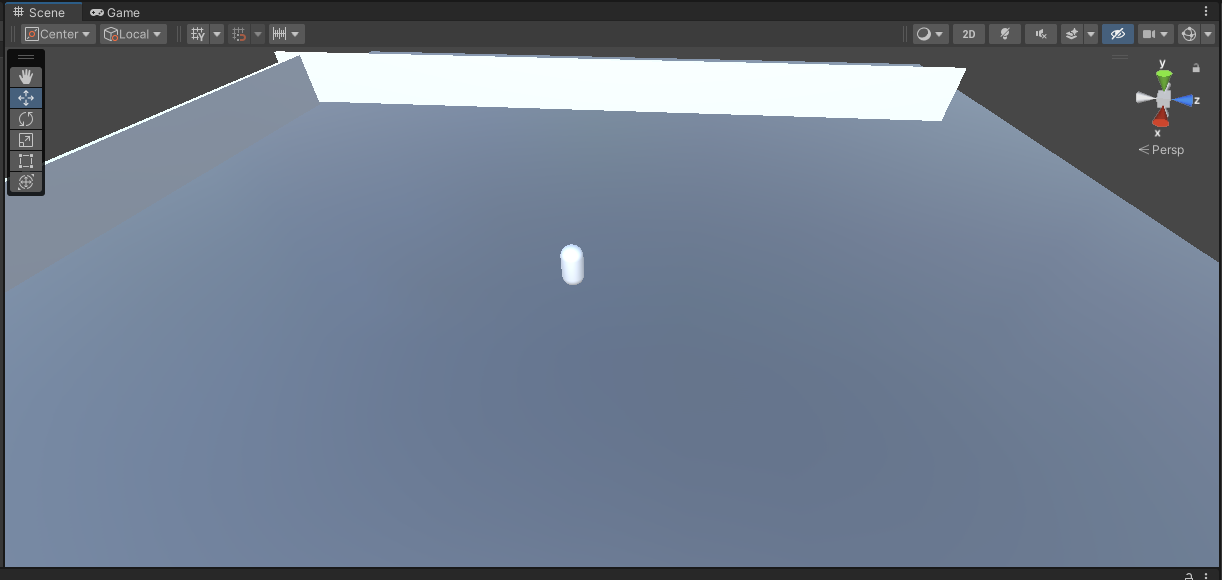
\includegraphics[width=.95\linewidth]{capsuleEnvironment.png}
    \caption{
        Initial test Environment
    }
    \label{figure 1}
\end{figure}
\begin{figure}
    \centering
    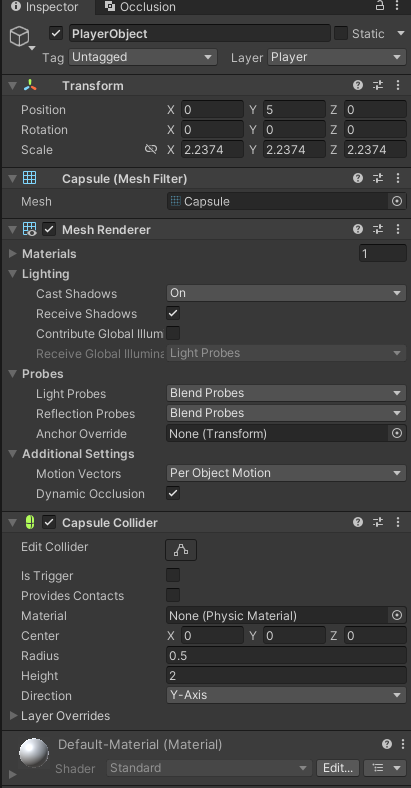
\includegraphics[width=.5\linewidth]{UnityInspector.png}
4    \caption{
        The Unity object inspector
    }
    \label{figure 2}
\end{figure}
The next step is to implement the movement of the player character in a new script PlayerMovement.cs. We add variables to keep track of movementSpeed, both horizontal and vertical input and a vector object for the calculated movement direction of the character. In order to calculate the movement direction the script takes the input from the keyboard, and adds together the vertical input and horizontal input into a vector. The script then takes that direction and adds the force to the rigidbody of the player model. Rigidbodies in unity are objects that interact with physics and can be added to any object. Adding a rigidbody to the player is useful as it allows the player to collide with the floor and other objects as well as allows the player to be affected by gravity.

After adding basic movement controls, the next important step is calculating drag, which is necessary for bunny hopping and creating responsive movement. As discussed in the introduction, drag only affects the player while on the ground, so a ground check must be implemented. The ground check is performed by sending a ray straight down from the player and checking if that ray touches the ground. If the ray makes contact, the player is grounded and the drag is subtracted from the movement speed. This also means that any surface the player should receive drag on must be tagged with the "ground" layer in the Unity GUI .

The final step of the tutorial I followed implemented jumping. Jumping involves an air movement speed multiplier, a jumpCooldown variable, and a boolean to check if the player is ready to jump. When the jump key is pressed and the player is grounded with no jump cooldown, the player's y velocity is reset so that the jump height is consistent and the upward velocity is added to the player's rigidbody.

While this script is sufficient for creating a basic movement system for a game, the way that velocity is calculated in the source engine is significantly more complicated. In order to understand and replicate counter-strike movement I used a detailed blog post that explains source engine movement and replicated that in Unity \cite{SourceImplementationBhop}. The largest difference in source movement is in how acceleration is calculated. Instead of directly limiting the velocity of a player, only the projection of the current velocity onto acceleration is limited. By changing the view direction of the player with mouse movement, the player's velocity can be kept above the maximum velocity set by the game.

To implement this additional functionality, I had to make some significant changes to the basic scripts. First I had to separate functions for movement in the air and movement on the ground, to support the velocity changes between the two with the new acceleration changes. Next I made a separate function for acceleration that calculates the projection velocity and the acceleration velocity separately and then checks if the player speed is greater than the max speed. I also had to incorporate the camera into the player object, as the mouse position now interacts more significantly with the movement calculations. 

\section{Metrics and Results}
The basic implementation of the movement system was relatively simple and the functionality present in my Unity project fully mimicked the functionality present in the tutorial. I was also able to extend this functionality which proves that the tutorial was successful in teaching the fundamentals of a movement system. In order to ensure that the grounded checks were working correctly I printed out the state every update. After implementing my version of the source movement system I created two walls in the game environment and timed how long it took the player to get from one wall to the other both walking and bunnyhopping shown in figure 3. The average time to reach the opposite wall walking was 4.45 seconds and the average time to reach the opposite wall bunnyhopping was 3.58 seconds. While user error is present in this procedure, there is a demonstrable effect on the speed of the player while bunnyhopping that proves the technique was implemented. 

While the gameplay of the final tutorial feels fluid, it does not exactly mimic the movement of counter-strike. The game feel is a very difficult attribute to measure emperically but is a vital part of my project and something that I will continue to refine. The source engine is different enough from unity that values for jump height, player speed and gravity can not be copied directly and must instead be replicated.
\begin{figure}
    \centering
    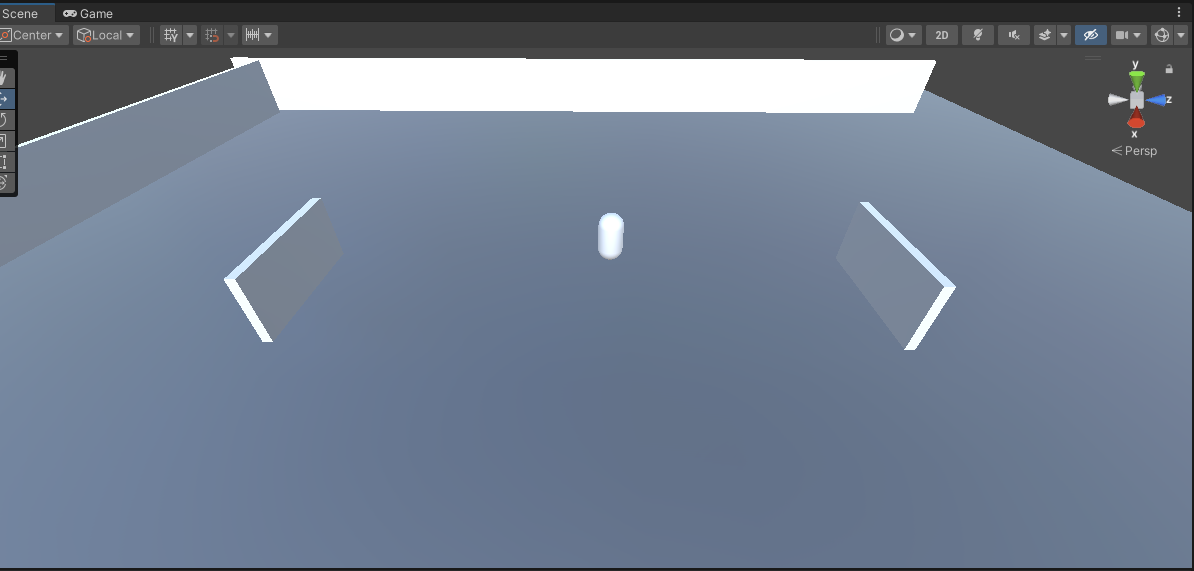
\includegraphics[width=.95\linewidth]{speedTest.png}
    \caption{
        The environment used to test bunnyhop speed
    }
    \label{figure 3}
\end{figure}

\section{Reflection}

Implementing an exact copy of a movement system into a different engine is difficult and learning to do so early will be crucial to my project. I had familiarity with the basic movement systems of Unity coming in to this project and the tutorial I followed was very helpful in expanding this knowledge and reminding me how components interact. In doing research for this project I also found that many other people have implemented movement from other games such as counter-strike into Unity. Access to all these resources should make implementation of an accurate source engine possible. While it would be possible to my project in the source engine and have a more direct copy of the movement in counter-strike but this would defeat my eventual goal of implementing movement systems from other games such as Valorant.

\printbibliography

\end{document}
